% Options for packages loaded elsewhere
\PassOptionsToPackage{unicode}{hyperref}
\PassOptionsToPackage{hyphens}{url}
%
\documentclass[
  12pt,
]{article}
\usepackage{lmodern}
\usepackage{amssymb,amsmath}
\usepackage{ifxetex,ifluatex}
\ifnum 0\ifxetex 1\fi\ifluatex 1\fi=0 % if pdftex
  \usepackage[T1]{fontenc}
  \usepackage[utf8]{inputenc}
  \usepackage{textcomp} % provide euro and other symbols
\else % if luatex or xetex
  \usepackage{unicode-math}
  \defaultfontfeatures{Scale=MatchLowercase}
  \defaultfontfeatures[\rmfamily]{Ligatures=TeX,Scale=1}
\fi
% Use upquote if available, for straight quotes in verbatim environments
\IfFileExists{upquote.sty}{\usepackage{upquote}}{}
\IfFileExists{microtype.sty}{% use microtype if available
  \usepackage[]{microtype}
  \UseMicrotypeSet[protrusion]{basicmath} % disable protrusion for tt fonts
}{}
\makeatletter
\@ifundefined{KOMAClassName}{% if non-KOMA class
  \IfFileExists{parskip.sty}{%
    \usepackage{parskip}
  }{% else
    \setlength{\parindent}{0pt}
    \setlength{\parskip}{6pt plus 2pt minus 1pt}}
}{% if KOMA class
  \KOMAoptions{parskip=half}}
\makeatother
\usepackage{xcolor}
\IfFileExists{xurl.sty}{\usepackage{xurl}}{} % add URL line breaks if available
\IfFileExists{bookmark.sty}{\usepackage{bookmark}}{\usepackage{hyperref}}
\hypersetup{
  pdftitle={Selective DNA and Protein Isolation from Marine Macrophyte Surfaces},
  hidelinks,
  pdfcreator={LaTeX via pandoc}}
\urlstyle{same} % disable monospaced font for URLs
\usepackage[margin=1.0in]{geometry}
\usepackage{graphicx,grffile}
\makeatletter
\def\maxwidth{\ifdim\Gin@nat@width>\linewidth\linewidth\else\Gin@nat@width\fi}
\def\maxheight{\ifdim\Gin@nat@height>\textheight\textheight\else\Gin@nat@height\fi}
\makeatother
% Scale images if necessary, so that they will not overflow the page
% margins by default, and it is still possible to overwrite the defaults
% using explicit options in \includegraphics[width, height, ...]{}
\setkeys{Gin}{width=\maxwidth,height=\maxheight,keepaspectratio}
% Set default figure placement to htbp
\makeatletter
\def\fps@figure{htbp}
\makeatother
\setlength{\emergencystretch}{3em} % prevent overfull lines
\providecommand{\tightlist}{%
  \setlength{\itemsep}{0pt}\setlength{\parskip}{0pt}}
\setcounter{secnumdepth}{-\maxdimen} % remove section numbering
\usepackage{times} % Times New Roman font
\usepackage[T1]{fontenc}

\usepackage[none]{hyphenat}

\usepackage{setspace}
\doublespacing
\setlength{\parskip}{1em}

\usepackage{lineno}

\usepackage{pdfpages}

\usepackage{indentfirst}

\usepackage[labelsep=period, labelfont=bf]{caption}
\renewcommand{\thefigure}{\arabic{figure}}
\renewcommand{\figurename}{Fig.}
\captionsetup{justification=raggedright,singlelinecheck=false}

\usepackage{pdflscape}
\newcommand{\blandscape}{\begin{landscape}}
\newcommand{\elandscape}{\end{landscape}}

\usepackage{siunitx}
\DeclareSIUnit\molar{\mole\per\cubic\deci\metre}
\DeclareSIUnit\Molar{\textsc{m}}
\DeclareSIUnit\cells{\text{cells}}

\usepackage{caption}
\captionsetup{justification=justified}

\usepackage{float}

\usepackage{xr}
\externaldocument[supp-]{supplementary}

\usepackage{txfonts}

\renewcommand{\figureautorefname}{Fig.}

\title{\textbf{Selective DNA and Protein Isolation from Marine Macrophyte
Surfaces}}
\author{}
\date{\vspace{-2.5em}}

\begin{document}
\maketitle

\vspace{20mm}

Marino Korlević\textsuperscript{1\(*\)}, Marsej
Markovski\textsuperscript{1}, Zihao Zhao\textsuperscript{2}, Gerhard J.
Herndl\textsuperscript{2,3}, Mirjana Najdek\textsuperscript{1}

1. Center for Marine Research, Ruđer Bošković Institute, Croatia

2. Department of Functional and Evolutionary Ecology, University of
Vienna, Austria

3. NIOZ, Department of Marine Microbiology and Biogeochemistry, Royal
Netherlands Institute for Sea Research, Utrecht University, The
Netherlands

\textsuperscript{\(*\)}To whom correspondence should be addressed:

Marino Korlević

G. Paliaga 5, 52210 Rovinj, Croatia

Tel.: +385 52 804 768

Fax: +385 52 804 780

e-mail:
\href{mailto:marino.korlevic@irb.hr}{\nolinkurl{marino.korlevic@irb.hr}}

Running title: DNA and protein isolation from macrophyte surfaces

\newpage
\linenumbers
\sisetup{mode=text}
\setlength\parindent{24pt}

\hypertarget{summary}{%
\subsection{Summary}\label{summary}}

Studies of unculturable microbes often combine methods based on DNA,
such as 16S rRNA sequencing and metagenomics, with methods that allow
insight into the metabolic status, such as metaproteomics. To apply
these techniques to the microbial community inhabiting the surfaces of
marine macrophytes it is advisable to perform, prior to the analysis, a
selective DNA and protein isolation so that the host material, present
in higher quantities, is not hampering the analysis. Two protocols, for
DNA and protein isolation, were adapted for selective extractions of DNA
and proteins from epiphytic communities inhabiting the surfaces of two
marine macrophytes: the seagrass \emph{Cymodocea nodosa} and the
macroalga \emph{Caulerpa cylindracea}. Protocols showed an almost
complete removal of the epiphytic community regardless of the sampling
season, station, settlement or host species. The obtained DNA was
suitable for metagenomic and 16S rRNA sequencing, while isolated
proteins could be identified by mass spectrometry, showing that
protocols can be used in 16S rRNA, metagenomic and metaproteomic
analysis. Low presence of host DNA and proteins, observed in isolated
samples, indicated a selective nature of the protocols. Furthermore, the
procedures are based on universally available laboratory chemicals
making the protocols widely applicable. Taken together, the adapted
protocols ensure an almost complete removal of the macrophyte epiphytic
community, are selective for microbes inhabiting macrophyte surfaces and
are providing DNA and proteins applicable in 16S rRNA sequencing,
metagenomics and metaproteomics.

\newpage

\hypertarget{introduction}{%
\subsection{Introduction}\label{introduction}}

Surfaces of marine macrophytes are inhabited by a diverse microbial
community whose structure and function are poorly understood (Egan
\emph{et al.}, 2013). As less than 1 \% of all prokaryotic species are
culturable, to study these organisms, molecular methods such as 16S rRNA
sequencing, metagenomics and metaproteomics are indispensable (Amann
\emph{et al.}, 1995; Su \emph{et al.}, 2012). Applying these techniques
requires an initial isolation step, with the purpose of obtaining high
quality DNA and proteins.

Biological material (i.e.~proteins and DNA) from pelagic microbial
communities is usually isolated by collecting cells onto filters and
subsequently isolating the aimed compound (Gilbert \emph{et al.}, 2009).
If a specific microbial size fraction is aimed sequential filtration is
applied (Massana \emph{et al.}, 1997; Andersson \emph{et al.}, 2010). In
contrast, obtaining biological materials from microorganism inhabiting
surfaces requires either a cell detachment procedure prior to isolation
or the host material is coextracted together with the targeted material.
Methods for separating microbial cells form the host include shaking of
host tissue (Gross \emph{et al.}, 2003; Nõges \emph{et al.}, 2010),
scraping of macrophyte surfaces (Uku \emph{et al.}, 2007) or the
application of ultrasonication (Weidner \emph{et al.}, 1996; Cai
\emph{et al.}, 2014). It was shown that shaking alone is not sufficient
to remove microbial cells, at least from plant root surfaces
(Richter-Heitmann \emph{et al.}, 2016). Manual separation methods, such
as scraping and brushing, are time consuming and subjective, as the
detachment efficiency depends on host tissue and the person performing
the procedure (Cai \emph{et al.}, 2014). Ultrasonication was proposed as
an alternative method as it is providing better results in terms of
detachment efficiency (Cai \emph{et al.}, 2014; Richter-Heitmann
\emph{et al.}, 2016). The downside of this procedure is that complete
cell removal was still not obtained and tissue disruption was observed
especially after the application of probe ultrasonication
(Richter-Heitmann \emph{et al.}, 2016). An alternative to these cell
detachment procedures is the isolation of targeted epiphytic compounds
together with host materials (Staufenberger \emph{et al.}, 2008; Jiang
\emph{et al.}, 2015). This procedure can lead to problems in the
following processing steps such as mitochondrial and chloroplast 16S
rRNA sequence contaminations from the host (Longford \emph{et al.},
2007; Staufenberger \emph{et al.}, 2008). In addition, when performing
metagenomics and metaproteomics host material can cause biased results
towards more abundant host DNA and proteins.

An alternative to these procedures is a direct isolation of the targeted
material by incubating macrophyte tissues in an extraction buffer. After
the incubation, the undisrupted host tissue is removed and the isolation
procedure continues, omitting host material contaminations. To our
knowledge the only procedure describing a direct and selective epiphytic
DNA isolation from the surfaces of marine macrophytes was provided by
Burke \emph{et al.} (2009). In contrast to previously described methods
this protocol enables an almost complete removal of the surface
community and it was used for 16S rRNA gene clone library construction
(Burke and Thomas \emph{et al.}, 2011) and metagenome sequencing (Burke
and Peter Steinberg \emph{et al.}, 2011). This method, thought providing
a selective isolation procedure, uses a rapid multienzyme cleaner (3M)
that is not available worldwide and without a known composition (Burke
\emph{et al.}, 2009). Also to our knowledge, no selective isolation
protocol for proteins from epiphytic communities inhabiting marine
macrophytes was established.

In the present study, we adapted a protocol widely used for DNA
isolation from filters (Massana \emph{et al.}, 1997) and a protocol used
for protein isolation from sediments (Chourey \emph{et al.}, 2010;
Hultman \emph{et al.}, 2015) for selective extractions of DNA and
proteins from epiphytic communities inhabiting the surfaces of two
marine macrophytes: the seagrass \emph{Cymodocea nodosa} and the
macroalga \emph{Caulerpa cylindracea}. In addition, we tested the
removal efficiency of the protocol and the suitability of obtained DNA
and proteins for 16S rRNA sequencing, metagenomics and metaproteomics.

\newpage

\hypertarget{results}{%
\subsection{Results}\label{results}}

To assess the removal efficiency of DNA and protein isolation procedures
leaves and thalli were examined under a confocal microscope before and
after treatments were performed. Developed procedures showed an almost
complete removal of the surface community of both, \emph{C. nodosa} and
\emph{C. cylindracea}. In addition, a similar removal efficiency was
observed for communities sampled in contrasting seasons, December 2017
(\autoref{confocal_december}) and June 2018 (\autoref{confocal_june}).
Also, no effect of station, settlement or isolation procedure (DNA or
protein) on the removal efficiency was observed (Figs.
\ref{confocal_december} and \ref{confocal_june}).

To evaluate if the obtained DNA is suitable to determine the microbial
community structure an Illumina sequencing of the V4 16S rRNA region was
performed. Sequencing yielded a total of 336,937 sequences after quality
curation and exclusion of eukaryotic, mitochondrial and no relative
sequences. The number of sequences classified as chloroplast was 97,328.
After excluding these sequences the total number of retrieved reads
dropped to 239,609, ranging from 22,587 to 52,958 sequences per sample
(\autoref{supp-nseq_notus}). Even when the highest sequencing effort was
applied the rarefaction curves did not level off which is commonly
observed in high-throughput 16S rRNA amplicon sequencing procedures
(\autoref{supp-rarefaction}). Sequence clustering at a similarity level
of 97 \si{\percent} yielded a total of 8,360 different OTUs. Taxonomic
classification of reads allowed for a macrophyte associated epiphytic
community determination that was mainly composed of:
\emph{Alphaproteobacteria} (14.9 ± 3.5 \si{\percent}),
\emph{Bacteroidota} (12.5 ± 2.4 \si{\percent}),
\emph{Gammaproteobacteria} (11.6 ± 4.3 \si{\percent}),
\emph{Desulfobacterota} (7.8 ± 7.4 \si{\percent}), \emph{Cyanobacteria}
(6.5 ± 4.7 \si{\percent}) and \emph{Planctomycetota} (2.9 ± 1.7
\si{\percent}) (\autoref{community}).

Primers used in this study, as in many other 16S rRNA amplicon
procedures, also amplified chloroplast 16S rRNA genes. We observed a
high proportion of chloroplast sequences in all analyzed samples (33.4 ±
9.4 \si{\percent}) (\autoref{community}). To determine if chloroplast
sequences originate from hosts or eukaryotic epiphytic organisms, we
exported SILVA classified chloroplast sequences and reclassified them
using the RDP (Ribosomal Database Project) training set that allows for
a more detailed chloroplast classification. The largest proportion of
sequences were classified as Bacillariophyta (89.7 ± 5.7 \si{\percent})
indicating that the DNA removal procedure did not coextract larger
quantities of host DNA (\autoref{chloroplast}). Chloroplast sequences
classified as Streptophyta constituted 3.3 ± 2.8 \si{\percent} of all
chloroplast sequences originating from \emph{C. nodosa} samples, while
sequences classified as Chlorophyta comprised only 0.02 ± 0.01
\si{\percent} of all chloroplast sequences associated with \emph{C.
cylindracea} samples.

To determine if the extracted DNA can be used for metagenomic sequencing
four samples containing epiphytic DNA were selected and shotgun
sequenced using an Illumina platform. Metagenomic sequencing yielded
from 207,149,524 to 624,029,930 sequence pairs
(\autoref{supp-metagenomic_statistics}). Obtained sequences were
successfully assembled into contigs whose L50 ranged from 654 to 1,011
bp. In addition, predicted coding sequences were successfully
functionally annotated (9,066,667 -- 20,256,215 annotated sequences;
\autoref{cog}) and taxonomically classified. Functional annotation
allowed for an assessment of the relative contribution of each COG
(Clusters of Orthologous Groups) functional category to the total number
of annotated coding sequences (\autoref{cog}a). Functional categories
containing the highest number of sequences were: C (Energy production
and conversion), E (Amino acid transport and metabolism), M (Cell
wall/membrane/envelope biogenesis), L (Replication, recombination and
repair) and P (Inorganic ion transport and metabolism). If host DNA was
coextracted with epiphytic it should be detected in larger proportions
in sequenced metagenomes. Indeed, no higher proportions of coding
sequences classified into phylum Streptophyta or Chlorophyta were
detected (\autoref{supp-metagenomic_taxonomy}). Sequenced metagenomic
DNA originating from the surface of \emph{C. nodosa} contained 1.3
\si{\percent} of coding sequences classified into the phylum
Streptophyta in December 2017 and 0.7 \si{\percent} in June 2018.
Furthermore, the summed RPKM (Reads Per Kilobase Million) of these
sequences constituted 1.7 \si{\percent} of total RPKM of all
successfully classified sequences in December 2017 and 1.1 \si{\percent}
in June 2018. Similar low proportions of host coding sequences were
detected in metagenomic samples originating from the surfaces of
\emph{C. cylindracea}. Of all successfully classified coding sequences
0.2 \si{\percent} were classified into Chlorophyta in December 2017 and
0.1 \si{\percent} in June 2018. A relatively higher proportion of these
sequences' RPKM than in the case of \emph{C. nodosa} was observed,
indicating a higher coextraction of host DNA in \emph{C. cylindracea}.
In December, the proportion of RPKM of sequences classified into
Chlorophyta was 8.2 \si{\percent}, while in June 2018 it reached 13.6
\si{\percent}.

To evaluate if the procedure for protein extraction is suitable for
metaproteomic analysis, obtained proteins were trypsin digested and
sequenced using a mass spectrometer. Obtained MS/MS spectra were
searched against a protein database from sequenced metagenomes. From
14,219 to 16,449 proteins were identified in isolated protein samples
(\autoref{cog}b). In addition, successful identification of proteins
allowed for an assessment of the relative contribution of each COG
functional category to the total number of identified proteins
(\autoref{cog}b). Functional categories containing the highest number of
identified proteins were: C (Energy production and conversion), G
(Carbohydrate transport and metabolism), P (Inorganic ion transport and
metabolism), O (Posttranslational modification, protein turnover,
chaperones) and E (Amino acid transport and metabolism). Isolated
proteins could derive from epiphytic organisms inhabiting the macrophyte
surface or from macrophyte tissue underlying them. The contribution of
proteins originating from host tissues was evaluated by identifying all
the proteins predicted to belong to any taxonomic group within the phyla
Streptophyta and Chlorophyta and by calculating their contribution to
the number and abundance of all identified proteins. On average,
proteins isolated from the surface of \emph{C. nodosa} contained 1.8 ±
0.06 \si{\percent} of proteins associated with Streptophyta,
contributing to 2.2 ± 0.8 \si{\percent} of total proteins. Similar to
metagenomes, proteins associated with Chlorophyta contributed more to
\emph{C. cylindracea} than proteins associated with Streptophyta to
\emph{C. nodosa}. Chlorophyta associated proteins comprised 5.2 ± 0.06
\si{\percent} of all identified proteins in \emph{C. cylindracea},
contributing to 19.2 ± 1.5 \si{\percent} of all protein abundances.

\hypertarget{discussion}{%
\subsection{Discussion}\label{discussion}}

The study of marine macrophyte epiphytic communities using culture
independent techniques, such as 16S rRNA analysis, metagenomics and
metaproteomics, requires an initial step of biological material
isolation. Methods that have been developed for selective isolation of
epiphytic biological material can be divided into two groups: (i)
procedures involving, prior to extraction, a cell detachment step such
as shaking (Gross \emph{et al.}, 2003; Nõges \emph{et al.}, 2010),
scraping (Uku \emph{et al.}, 2007) and ultrasonication (Weidner \emph{et
al.}, 1996; Cai \emph{et al.}, 2014) and (ii) procedures involving a
host tissue incubation aiming at direct lysis of epiphytic microbial
cells (Burke \emph{et al.}, 2009). Protocols that include a cell
detachment procedure do not provide complete cell removal (Cai \emph{et
al.}, 2014; Richter-Heitmann \emph{et al.}, 2016) and in the case of
probe ultrasonication tissue disruption can also be observed
(Richter-Heitmann \emph{et al.}, 2016). Though, host tissue incubation
procedures provide an almost complete cell removal and selective
isolation, existing protocols like the one developed for DNA isolation
by Burke \emph{et al.} (2009) use in the extraction buffer a rapid
multienzyme cleaner (3M) not available worldwide and without a known
composition (Burke \emph{et al.}, 2009). To circumvent these problems we
developed and tested two protocols for selective DNA and protein
isolation from marine macrophyte epiphytic communities.

To test if the developed DNA and protein isolation procedures could be
applied on a variety of macrophyte species we selected \emph{C. nodosa}
and \emph{C. cylindracea} as representatives of seagrass and macroalgal
species, on which the procedures were tested. These species especially
differ morphologically. While \emph{C. nodosa} leaves are flat, \emph{C.
cylindracea} thallus is composed of uneven surfaces (Kuo and den Hartog,
2001; Verlaque \emph{et al.}, 2003). The developed procedures showed an
almost complete removal of epiphytic cells from the surfaces of both
species comparable to the result of Burke \emph{et al.} (2009) and
indicating that structural differences do not impact the removal
efficiency. In addition, isolation protocols were tested in two
contrasting season as it is known that macrophytes are harboring more
algal epiphytes during autumn and winter (Reyes and Sansón, 2001). No
differences in the removal efficiency was observed between seasons
suggesting that protocols can be used on macrophyte samples retrieved
throughout the year. Also, no removal differences were observed on
samples derived from the same host but from different localities or
settlements demonstrating the stability of the protocol in cell removal
efficiency.

Successful amplification and sequencing of the V4 16S rRNA gene region
proved that the isolated DNA can be used to estimate the microbial
epiphytic diversity. Taxonomic groups detected in this step can also be
often found in epiphytic communities associated with other macrophytes
(Burke and Thomas \emph{et al.}, 2011; Morrissey \emph{et al.}, 2019). A
problem often encountered in studies focusing on epiphytic communities
is the presence of large proportions of chloroplast 16S rRNA sequences
in the pool of amplified molecules, especially if the epiphytic DNA was
isolated without prior selection (Staufenberger \emph{et al.}, 2008).
These sequences can derive from host chloroplasts or from eukaryotic
epiphytic chloroplast DNA. Although the proportion of obtained
chloroplast 16S rRNA sequences in our samples was substantial they
derived almost exclusively from eukaryotic epiphytes. High proportion of
chloroplast 16S rRNA sequences in studies applying selective procedures
that include direct cellular lysis on host surfaces were observed before
(Michelou \emph{et al.}, 2013). It is possible that chloroplast specific
sequences even in these studies are originating from eukaryotic
epiphytic cells and not host chloroplast. Indeed, it is common during
16S rRNA profiling of pelagic microbial communities to observe high
proportions of chloroplast sequences (Gilbert \emph{et al.}, 2009;
Korlević \emph{et al.}, 2016). In addition, a very low proportion of
chloroplast 16S rRNA sequences in samples originating from \emph{C.
cylindracea} in comparison to \emph{C. nodosa} could be explained by the
presence of three introns in the gene for 16S rRNA in some members of
the genus \emph{Caulerpa} that could hamper the amplification process
(Lam and Lopez-Bautista, 2016).

Beside 16S rRNA sequencing high quality DNA is needed for metagenomics.
The obtained number of metagenomic sequences and assembly statistics
were comparable to metagenomes and metatranscriptomes derived from
similar surface associated communities (Crump \emph{et al.}, 2018; Cúcio
\emph{et al.}, 2018). In addition, functional annotation of predicted
coding sequences to COG functional categories showed that the obtained
metagenomes can be used to determine the metabolic capacity of surface
associated communities (Leary \emph{et al.}, 2014; Cúcio \emph{et al.},
2018). The proportion of coding sequences, including their RPKM,
originating from \emph{C. nodosa} metagenomes and classified as
Streptophyta was low indicating a good selectivity of the isolation
procedure towards epiphytic cells. In the case of DNA samples isolated
from the surface of \emph{C. cylindracea} the proportion of Chlorophyta
coding sequences was also low but their RPKM was higher than in the case
of \emph{C. nodosa}. One of the causes for this elevated RPKM of
Chlorophyta sequences in \emph{C. cylindracea} could lay in tissue
structure differences between these two host species. While \emph{C.
nodosa} leaves are composed of individual cells, the thallus of \emph{C.
cylindracea} is, like in other siphonous algal species, composed of a
single large multinucleate cell (Coneva and Chitwood, 2015). The absence
of individual cells in \emph{C. cylindracea} could cause a leakage of
genetic material into the extraction buffer causing an elevated presence
of host sequences in metagenomic data.

To obtain an insight into the metabolic status of uncultivated members,
a metaproteomic approach is required (Saito \emph{et al.}, 2019). The
applied protocol for epipyhtic protein isolation followed by a
metaproteomic analysis identified between 14,219 and 16,449 proteins,
which is higher than previously reported for e.g.~soils (Chourey
\emph{et al.}, 2010; Hultman \emph{et al.}, 2015), seawater (Williams
\emph{et al.}, 2012) and biofilms (Leary \emph{et al.}, 2014). The
functional annotation of identified proteins into COG functional
categories showed that the protein isolation procedure can be used to
assess the metabolic status of the macrophyte epiphytic community (Leary
\emph{et al.}, 2014). Similar to metagenomes, the number of identified
proteins, including their abundances, associated with Streptophyta in
\emph{C. nodosa} samples were low indicating that the procedure is
selective for epiphytic cell proteins. In addition, a higher number of
identified proteins, and especially their abundances, associated with
Chlorophyta was observed in \emph{C. cylindracea} samples. The cause of
this elevated presence of Chlorophyta associated proteins can be, as in
the case of the DNA isolation procedure, explained by the absence of
individual cells in this siphonous alga (Coneva and Chitwood, 2015).

In conclusion, the developed protocols for DNA and protein isolation
from macrophyte surfaces are providing an almost complete removal of the
epiphytic community and are shown to ensure removal from both, \emph{C.
nodosa} and \emph{C. cylindracea}, in different seasons. Also, the
obtained DNA and proteins are suitable for 16S rRNA sequencing,
metagenomics and metaproteomics, while the obtained material contains
low quantities of host DNA or proteins making the procedures epiphyte
selective. Furthermore, the procedures are based on universally
available laboratory chemicals making the protocols widely applicable.

\newpage

\hypertarget{experimental-procedures}{%
\subsection{Experimental procedures}\label{experimental-procedures}}

\hypertarget{sampling}{%
\subsubsection{Sampling}\label{sampling}}

Leaves of \emph{C. nodosa} were sampled in a \emph{C. nodosa} meadow in
the Bay of Saline (\ang{45;7;5} N, \ang{13;37;20} E) and in a \emph{C.
nodosa} meadow invaded by \emph{C. cylindracea} in the proximity of the
village of Funtana (Bay of Funtana; \ang{45;10;39} N, \ang{13;35;42} E).
Thalli of \emph{C. cylindracea} were sampled in the same \emph{C.
nodosa} invaded meadow in the Bay of Funtana and on a locality of only
\emph{C. cylindracea} located in the proximity of the invaded meadow.
Leaves and thalli for 16S rRNA analysis, metagenomics and metaproteomics
were collected in two contrasting seasons, on 4 December 2017 (16S rRNA
analysis and metaproteomics), 14 December 2017 (metagenomics) and 18
June 2018 (16S rRNA analysis, metagenomics and metaproteomics). During
spring 2018 the \emph{C. nodosa} meadow in the Bay of Saline decayed to
an extent that no leaves could be retrieved (Najdek \emph{et al.},
2020). In addition, as not enough DNA for both metagenomic and 16S RNA
analysis were obtained during the sampling on 4 December 2017, an
additional sampling on 14 December 2017 was carried out in the Bay of
Funtana. Leaves and thalli were collected by diving and transported to
the laboratory in containers placed on ice and filled with site
seawater. Upon arrival to the laboratory, \emph{C. nodosa} leaves were
cut into sections of 1 -- 2 \si{\cm}, while \emph{C. cylindracea} thalli
were cut into 5 -- 8 \si{\cm} long sections. Leaves and thalli were
washed three times with sterile artificial seawater (ASW) to remove
loosely attached microbial cells.

\hypertarget{dna-isolation}{%
\subsubsection{DNA isolation}\label{dna-isolation}}

The DNA was isolated according to the protocol for isolation from
filters described in Massana \emph{et al.} (1997). This protocol was
modified and adapted for microbial DNA isolation from macrophyte
surfaces as described below. 5 \si{\ml} of lysis buffer (40
\si{\milli\Molar} EDTA, 50 \si{\milli\Molar} Tris-HCl, 0.75 \si{\Molar}
sucrose; pH 8.3) was added to 1 \si{\g} wet weight of leaves or 2
\si{\g} wet-weight of thalli. For every sample duplicate isolations were
performed. Lysozyme was added (final concentration 1 \si{\mg\per\ml})
and the mixture was incubated at 37 \si{\degreeCelsius} for 30
\si{\minute}. Subsequently, proteinase K (final concentration 0.5
\si{\mg\per\ml}) and SDS (final concentration 1 \si{\percent}) were
added and the samples were incubated at 55 \si{\degreeCelsius} for 2
\si{\hour}. Following the incubation, tubes were vortexed for 10
\si{\minute} and the mixture containing lyzed epiphytic cells was
separated from host leaves or thalli by transferring the solution into a
clean tube. The lysate was extracted twice with a mixture of
phenol:chloroform:isoamyl alcohol (25:24:1; pH 8) and once with
chloroform:isoamyl alcohol (24:1). After each organic solvent mixture
addition tubes were slightly vortexed and centrifuged at 4,500 × g for
10 \si{\minute}. Following each centrifugation aqueous phases were
retrieved. After the final extraction 1/10 of chilled 3 \si{\Molar}
sodium acetate (pH 5.2) was added. DNA was precipitated by adding 1
volume of chilled isopropanol, incubating the mixtures overnight at
\num{-20} °C and centrifuging at 16,000 × g and 4 \si{\degreeCelsius}
for 20 \si{\minute}. The pellet was washed twice with 1 \si{\ml} of
chilled 70 \si{\percent} ethanol and centrifuged after each washing step
at 20,000 × g and 4 \si{\degreeCelsius} for 10 \si{\minute}. After the
first washing step duplicate pellets form the same sample were pooled
and transferred to a clean 1.5 \si{\ml} tube. The dried pellet was
resuspended in 100 \si{\ul} of deionized water.

\hypertarget{illumina-16s-rrna-sequencing}{%
\subsubsection{Illumina 16S rRNA
sequencing}\label{illumina-16s-rrna-sequencing}}

An aliquot of isolated DNA was treated with RNase A (final concentration
200 \si{\ug\per\ml}) for 2 \si{\hour} at 37 \si{\degreeCelsius}. The DNA
concentration was determined using the Quant-iT PicoGreen dsDNA Assay
Kit (Invitrogen, USA) according to the manufacturer's instructions and
diluted to 1 \si{\ng\per\ul}. The V4 region of the 16S rRNA gene was
amplified using a two-step PCR procedure. In the first PCR the 515F
(5'-GTGYCAGCMGCCGCGGTAA-3') and 806R (5'-GGACTACNVGGGTWTCTAAT-3')
primers from the Earth Microbiome Project
(\url{http://press.igsb.anl.gov/earthmicrobiome/protocols-and-standards/16s/})
were used to amplify the target region (Caporaso \emph{et al.}, 2012;
Apprill \emph{et al.}, 2015; Parada \emph{et al.}, 2016). These primers
contained on their 5' end a tagged sequence. Each sample was amplified
in four parallel 25 \si{\ul} reactions of which each contained: 1 × Q5
Reaction Buffer , 0.2 \si{\milli\Molar} of dNTPmix, 0.7 \si{\mg\per\ml}
BSA (Bovine Serum Albumin), 0.2 \si{\micro\Molar} of forward and reverse
primers, 0.5 U of Q5 High-Fidelity DNA Polymerase (New England Biolabs,
USA) and 5 \si{\ng} of DNA template. Cycling conditions were: initial
denaturation at 94 \si{\degreeCelsius} for 3 \si{\minute}, 20 cycles of
denaturation at 94 \si{\degreeCelsius} for 45 \si{\s}, annealing at 50
\si{\degreeCelsius} for 60 \si{\s} and elongation at 72
\si{\degreeCelsius} for 90 \si{\s}, finalized by an elongation step at
72 \si{\degreeCelsius} for 10 \si{\minute}. The four parallel reactions
volumes were pooled and PCR products were purified using the GeneJET PCR
Purification Kit (Thermo Fisher Scientific, USA) according to the
manufacturer's instructions and following the protocol that included
isopropanol addition for better small DNA fragment yield. The column was
eluted in 30 \si{\ul} of deionized water. Purified PCR products were
sent for Illumina MiSeq sequencing (2 × 250 bp) at IMGM Laboratories,
Martinsried, Germany. Before sequencing at IMGM, the second PCR
amplification of the two-step PCR procedure was performed using primers
targeting the tagged region incorporated in the first PCR. In addition,
these primers contained adapter and sample-specific index sequences. The
second PCR was carried out for 8 cycles. Beside samples, a positive and
negative control were sequenced. A negative control was comprised of
four parallel PCR reactions without DNA template, while for a positive
control a mock community composed of evenly mixed DNA material
originating from 20 bacterial strains (ATCC MSA-1002, ATCC, USA) was
used. Partial 16S rRNA sequences obtained in this study have been
deposited in the European Nucleotide Archive (ENA) at EMBL-EBI under
accession numbers SAMEA6786270, SAMEA6648792 -- SAMEA6648794,
SAMEA6648809 -- SAMEA6648811.

Obtained sequences were analyzed on the computer cluster Isabella
(University Computing Center, University of Zagreb) using mothur
(version 1.43.0) (Schloss \emph{et al.}, 2009) according to the MiSeq
Standard Operating Procedure (MiSeq SOP;
\url{https://mothur.org/wiki/MiSeq_SOP}) (Kozich \emph{et al.}, 2013)
and recommendations given from the Riffomonas project to enhance data
reproducibility (\url{http://www.riffomonas.org/}). For alignment and
classification of sequences the SILVA SSU Ref NR 99 database (release
138; \url{http://www.arb-silva.de}) was used (Quast \emph{et al.}, 2013;
Yilmaz \emph{et al.}, 2014). Sequences classified as chloroplasts by
SILVA were exported and reclassifed using mothur and the RDP
(\url{http://rdp.cme.msu.edu/}) training set (version 16) reference
files adapted for mothur (Cole \emph{et al.}, 2014). In comparison to
SILVA, RDP allows a more detailed classification of chloroplast
sequences. Pipeline data processing and visualization was done using R
(version 3.6.0) (R Core Team, 2019), package tidyverse (version 1.3.0)
(Wickham \emph{et al.}, 2019) and multiple other packages (Xie, 2014,
2015, 2020; Neuwirth, 2014; Xie \emph{et al.}, 2018; Wilke, 2018; Y.
Xie, 2019b, 2019a; Allaire \emph{et al.}, 2019; Zhu, 2019; Bengtsson,
2020). The detailed analysis procedure including the R Markdown file for
this paper are available as a GitHub repository
(\url{https://github.com/mkorlevic/Korlevic_SelectiveRemoval_EnvironMicrobiol_2020}).
Based on the ATCC MSA-1002 mock community included in the analysis a
sequencing error rate of 0.009 \si{\percent} was determined, which is in
line with previously reported values for next-generation sequencing data
(Kozich \emph{et al.}, 2013; Schloss \emph{et al.}, 2016). In addition,
the negative control processed together with the samples yielded only 2
sequences after sequence quality curation.

\hypertarget{metagenomics}{%
\subsubsection{Metagenomics}\label{metagenomics}}

Four DNA samples were selected and sent on dry ice to IMGM Laboratories,
Martinsried, Germany for metagenomic sequencing. DNA was purified using
AMPure XP Beads (Beckman Coulter, USA) applying a bead:DNA ratio of 1:1
(v/v), quantified with a Qubit dsDNA HS Assay Kit (Thermo Fisher
Scientific, USA) and check for integrity on a 1 \si{\percent} agarose
gel. Metagenomic sequencing libraries were generated from 300 \si{\ng}
of input DNA using a NEBNext Ultra II FS DNA Library Prep Kit for
Illumina (New England Biolabs, USA) according to the manufacturer's
instructions. Fragments were selected (500 -- 700 bp) using AMPure XP
Beads, PCR enriched for 3 -- 5 cycles and quality controlled. Libraries
generated from different DNA samples were pooled and sequenced on an
Illumina NovaSeq 6000 sequencing system (2 × 250 bp).

Obtained sequences were analyzed on a Life Science Compute Cluster
(LiSC) (CUBE -- Computational Systems Biology, University of Vienna).
Individual sequences were assembled using MEGAHIT (version 1.1.2) (Li
\emph{et al.}, 2015) under default settings. Putative genes were
predicted from contings longer than 200 bp using Prodigal (version
2.6.3) (Hyatt \emph{et al.}, 2010) in metagenome mode (-p meta).
Abundances of predicted genes were expressed as Reads Per Kilobase
Million (RPKM) and calculated using the BWA algorithm (version 0.7.16a)
(Li and Durbin, 2009). All predicted genes were functionally annotated
using the eggNOG-mapper (Huerta-Cepas \emph{et al.}, 2017) and eggNOG
database (version 5.0) (Huerta-Cepas \emph{et al.}, 2019). Sequence
taxonomy classification was determined using the lowest common ancestor
algorithm adapted from DIAMOND (version 0.8.36) (Buchfink \emph{et al.},
2015) and by searching against the NCBI non-redundant database (NR). To
determine phylogeny the top 10 \si{\percent} hits with an e-value
\textless{} 1 × 10\textsuperscript{-5} were used (-\/-top 10). Sequence
renaming, coverage information computing and metagenomic statistics
calculations were performed using software tools from BBTools
(\url{https://jgi.doe.gov/data-and-tools/bbtools}). Metagenomic
sequences obtained in this study have been deposited in the European
Nucleotide Archive (ENA) at EMBL-EBI under accession numbers \textbf{TO
BE ADDED}.

\hypertarget{protein-isolation}{%
\subsubsection{Protein isolation}\label{protein-isolation}}

Proteins were isolated according to the protocol for protein isolation
from soil described in Chourey \emph{et al.} (2010) and modified by
Hultman \emph{et al.} (2015). This protocol was further modified and
adapted for microbial protein isolation from macrophyte surfaces as
described below. 20 \si{\ml} of protein extraction buffer (4
\si{\percent} SDS, 100 \si{\milli\Molar} Tris-HCl {[}pH 8.0{]}) was
added to 5 \si{\g} wet weight of leaves or 10 \si{\g} wet weight of
thalli. The mixture was incubated in boiling water for 5 \si{\minute},
vortexed for 10 \si{\minute} and incubated again in boiling water for 5
\si{\minute}. After a brief vortex the lysate was transferred to a clean
tube separating the host leaves or thalli from the mixture containing
lyzed epiphytic cells. Dithiothreitol (DTT; final concentration 24
\si{\milli\Molar}) was added and proteins were precipitated with chilled
100 \si{\percent} trichloroacetic acid (TCA; final concentration 20
\si{\percent}) overnight at \num{-20} °C. Precipitated proteins were
centrifuged at 10,000 × g and 4 \si{\degreeCelsius} for 40 \si{\minute}.
The obtained protein pellet was washed three times with chilled acetone.
During the first washing step the pellet was transferred to a clean 1.5
\si{\ml} tube. After each washing step samples were centrifuged at
20,000 × g and 4 \si{\degreeCelsius} for 5 \si{\minute}. Dried pellets
were stored at \num{-80} °C until further analysis.

\hypertarget{metaproteomics}{%
\subsubsection{Metaproteomics}\label{metaproteomics}}

Isolated proteins were whole trypsin digested using the FASP
(filter-aided sample preparation) Protein Digestion Kit (Expedeon, UK)
according to the manufacturer's instructions with small modifications
(Wiśniewski \emph{et al.}, 2009). Before the solution was loaded to the
column, protein pellets were solubilized in a urea sample buffer
included in the kit amended with DTT (final concentration 100
\si{\milli\Molar}) for 45 \si{\minute} at room temperature and
centrifuged at 20,000 × g for 2 -- 5 \si{\minute} at room temperature to
remove larger particles. The first washing step after protein solution
loading was repeated twice. In addition, centrifugation steps were
prolonged if the column was clogged. Trypsin digestion was performed on
column filters at 37 \si{\degreeCelsius} overnight for 18 \si{\hour}.
The final filtrate containing peptides was acidified with 1
\si{\percent} (final concentration) trifluoroacetic acid, freezed at
\num{-80} \si{\degreeCelsius} for 15 \si{\minute}, lyophilized and sent
to the Vienna Metabolomics Center (University of Vienna) for
metaproteomic analysis. Peptides were resuspended in 1 \si{\percent}
(final concentration) trifluoroacetic acid (TFA), desalted using the
Pierce C18 Tips (Thermo Fisher Scientific, USA) according to the
manufacturer's instructions and sequenced on a Q Exactive Hybrid
Quadrupole-Orbitrap Mass Spectrometer (Thermo Fisher Scientific, USA).
Obtained MS/MS spectra were searched against a protein database composed
of combined sequenced metagenomes using SEQUEST-HT engines and validated
with Percolator in Proteome Discoverer 2.1 (Thermo Fisher Scientific,
USA). The target-decoy approach was used to reduce the probability of
false peptide identification. Results whose false discovery rate at the
peptide level was \SI{< 1}{\percent} were kept. For protein
identification a minimum of two peptides and one unique peptide were
required. For protein quantification, a chromatographic peak area-based
free quantitative method was applied.

\hypertarget{confocal-microscopy}{%
\subsubsection{Confocal microscopy}\label{confocal-microscopy}}

Host leaves and thalli from DNA and protein isolation steps were washed
seven times in deionized water and fixed with formaldehyde (final
concentration \textasciitilde{} 3 \si{\percent}). In addition,
nontreated leaves and thalli, washed three times in ASW to remove
loosely attached microbial cells, were fixed in the same concentration
of formaldehyde and used as a positive control. For long therm storage,
fixed leaves and thalli were immersed in a mixture of phosphate-buffered
saline (PBS) and ethanol (1:1) and stored at \num{-20}
\si{\degreeCelsius}. Treated and untreated segemnts of leaves and thalli
were stained in a 2 × solution of SYBR Green I and examined under a
Leica TCS SP8 X FLIM confocal microscope (Leica Microsystems, Germany).

\hypertarget{acknowledgements}{%
\subsection{Acknowledgements}\label{acknowledgements}}

This work was founded by the Croatian Science Foundation through the
MICRO-SEAGRASS project (IP-2016-06-7118). We would like to thank
Margareta Buterer for technical support, Paolo Paliaga for help during
sampling, Lucija Horvat for technical support in confocal microscopy and
Dušica Vujaklija for help in accessing the confocal microscope. In
addition, we would like to thank the University Computing Center of the
University of Zagreb for access to the computer cluster Isabella and
CUBE -- Computational Systems Biology of the University of Vienna for
access to the Life Science Compute Cluster (LiSC).

\newpage

\hypertarget{references}{%
\subsection{References}\label{references}}

\hypertarget{refs}{}
\leavevmode\hypertarget{ref-Allaire2019}{}%
Allaire, J.J., Xie, Y., McPherson, J., Luraschi, J., Ushey, K., Atkins,
A., et al. (2019) rmarkdown: Dynamic documents for R.

\leavevmode\hypertarget{ref-Amann1995}{}%
Amann, R.I., Ludwig, W., and Schleifer, K.H. (1995) Phylogenetic
identification and \emph{in situ} detection of individual microbial
cells without cultivation. \emph{Microbiol Rev} \textbf{59}: 143--169.

\leavevmode\hypertarget{ref-Andersson2010}{}%
Andersson, A.F., Riemann, L., and Bertilsson, S. (2010) Pyrosequencing
reveals contrasting seasonal dynamics of taxa within Baltic Sea
bacterioplankton communities. \emph{ISME J} \textbf{4}: 171--181.

\leavevmode\hypertarget{ref-Apprill2015}{}%
Apprill, A., McNally, S., Parsons, R., and Weber, L. (2015) Minor
revision to V4 region SSU rRNA 806R gene primer greatly increases
detection of SAR11 bacterioplankton. \emph{Aquat Microb Ecol}
\textbf{75}: 129--137.

\leavevmode\hypertarget{ref-Bengtsson2020}{}%
Bengtsson, H. (2020) matrixStats: Functions that apply to rows and
columns of matrices (and to vectors).

\leavevmode\hypertarget{ref-Buchfink2015}{}%
Buchfink, B., Xie, C., and Huson, D.H. (2015) Fast and sensitive protein
alignment using DIAMOND. \emph{Nat Methods} \textbf{12}: 59--60.

\leavevmode\hypertarget{ref-Burke2009}{}%
Burke, C., Kjelleberg, S., and Thomas, T. (2009) Selective extraction of
bacterial DNA from the surfaces of macroalgae. \emph{Appl Environ
Microbiol} \textbf{75}: 252--256.

\leavevmode\hypertarget{ref-Burke2011}{}%
Burke, C., Steinberg, P., Rusch, D., Kjelleberg, S., and Thomas, T.
(2011) Bacterial community assembly based on functional genes rather
than species. \emph{Proc Natl Acad Sci U S A} \textbf{108}:
14288--14293.

\leavevmode\hypertarget{ref-Burke2011a}{}%
Burke, C., Thomas, T., Lewis, M., Steinberg, P., and Kjelleberg, S.
(2011) Composition, uniqueness and variability of the epiphytic
bacterial community of the green alga \emph{Ulva australis}. \emph{ISME
J} \textbf{5}: 590--600.

\leavevmode\hypertarget{ref-Cai2014}{}%
Cai, X., Gao, G., Yang, J., Tang, X., Dai, J., Chen, D., and Song, Y.
(2014) An ultrasonic method for separation of epiphytic microbes from
freshwater submerged macrophytes. \emph{J Basic Microbiol} \textbf{54}:
758--761.

\leavevmode\hypertarget{ref-Caporaso2012}{}%
Caporaso, J.G., Lauber, C.L., Walters, W.A., Berg-Lyons, D., Huntley,
J., Fierer, N., et al. (2012) Ultra-high-throughput microbial community
analysis on the Illumina HiSeq and MiSeq platforms. \emph{ISME J}
\textbf{6}: 1621--1624.

\leavevmode\hypertarget{ref-Chourey2010}{}%
Chourey, K., Jansson, J., VerBerkmoes, N., Shah, M., Chavarria, K.L.,
Tom, L.M., et al. (2010) Direct cellular lysis/protein extraction
protocol for soil metaproteomics. \emph{J Proteome Res} \textbf{9}:
6615--6622.

\leavevmode\hypertarget{ref-Cole2014}{}%
Cole, J.R., Wang, Q., Fish, J.A., Chai, B., McGarrell, D.M., Sun, Y., et
al. (2014) Ribosomal Database Project: Data and tools for high
throughput rRNA analysis. \emph{Nucleic Acids Res} \textbf{42}:
D633--D642.

\leavevmode\hypertarget{ref-Coneva2015}{}%
Coneva, V. and Chitwood, D.H. (2015) Plant architecture without
multicellularity: Quandaries over patterning and the soma-germline
divide in siphonous algae. \emph{Front Plant Sci} \textbf{6}: 287.

\leavevmode\hypertarget{ref-Crump2018}{}%
Crump, B.C., Wojahn, J.M., Tomas, F., and Mueller, R.S. (2018)
Metatranscriptomics and amplicon sequencing reveal mutualisms in
seagrass microbiomes. \emph{Front Microbiol} \textbf{9}: 388.

\leavevmode\hypertarget{ref-Cucio2018}{}%
Cúcio, C., Overmars, L., Engelen, A.H., and Muyzer, G. (2018)
Metagenomic analysis shows the presence of bacteria related to
free-living forms of sulfur-oxidizing chemolithoautotrophic symbionts in
the rhizosphere of the seagrass \emph{Zostera marina}. \emph{Front Mar
Sci} \textbf{5}: 171.

\leavevmode\hypertarget{ref-Egan2013}{}%
Egan, S., Harder, T., Burke, C., Steinberg, P., Kjelleberg, S., and
Thomas, T. (2013) The seaweed holobiont: Understanding seaweed-bacteria
interactions. \emph{FEMS Microbiol Rev} \textbf{37}: 462--476.

\leavevmode\hypertarget{ref-Gilbert2009}{}%
Gilbert, J.A., Field, D., Swift, P., Newbold, L., Oliver, A., Smyth, T.,
et al. (2009) The seasonal structure of microbial communities in the
Western English Channel. \emph{Environ Microbiol} \textbf{11}:
3132--3139.

\leavevmode\hypertarget{ref-Gross2003}{}%
Gross, E.M., Feldbaum, C., and Graf, A. (2003) Epiphyte biomass and
elemental composition on submersed macrophytes in shallow eutrophic
lakes. \emph{Hydrobiologia} \textbf{506-509}: 559--565.

\leavevmode\hypertarget{ref-Huerta-Cepas2017}{}%
Huerta-Cepas, J., Forslund, K., Coelho, L.P., Szklarczyk, D., Jensen,
L.J., von Mering, C., and Bork, P. (2017) Fast genome-wide functional
annotation through orthology assignment by eggNOG-mapper. \emph{Mol Biol
Evol} \textbf{34}: 2115--2122.

\leavevmode\hypertarget{ref-Huerta-Cepas2019}{}%
Huerta-Cepas, J., Szklarczyk, D., Heller, D., Hernández-Plaza, A.,
Forslund, S.K., Cook, H., et al. (2019) eggNOG 5.0: A hierarchical,
functionally and phylogenetically annotated orthology resource based on
5090 organisms and 2502 viruses. \emph{Nucleic Acids Res} \textbf{47}:
D309--D314.

\leavevmode\hypertarget{ref-Hultman2015}{}%
Hultman, J., Waldrop, M.P., Mackelprang, R., David, M.M., McFarland, J.,
Blazewicz, S.J., et al. (2015) Multi-omics of permafrost, active layer
and thermokarst bog soil microbiomes. \emph{Nature} \textbf{521}:
208--212.

\leavevmode\hypertarget{ref-Hyatt2010}{}%
Hyatt, D., Chen, G.-L., LoCascio, P.F., Land, M.L., Larimer, F.W., and
Hauser, L.J. (2010) Prodigal: Prokaryotic gene recognition and
translation initiation site identification. \emph{BMC Bioinformatics}
\textbf{11}: 119.

\leavevmode\hypertarget{ref-Jiang2015}{}%
Jiang, Y.-F., Ling, J., Dong, J.-D., Chen, B., Zhang, Y.-Y., Zhang,
Y.-Z., and Wang, Y.-S. (2015) Illumina-based analysis the microbial
diversity associated with \emph{Thalassia hemprichii} in Xincun Bay,
South China Sea. \emph{Ecotoxicology} \textbf{24}: 1548--56.

\leavevmode\hypertarget{ref-Korlevic2016}{}%
Korlević, M., Šupraha, L., Ljubešić, Z., Henderiks, J., Ciglenečki, I.,
Dautović, J., and Orlić, S. (2016) Bacterial diversity across a highly
stratified ecosystem: A salt-wedge Mediterranean estuary. \emph{Syst
Appl Microbiol} \textbf{39}: 398--408.

\leavevmode\hypertarget{ref-Kozich2013}{}%
Kozich, J.J., Westcott, S.L., Baxter, N.T., Highlander, S.K., and
Schloss, P.D. (2013) Development of a dual-index sequencing strategy and
curation pipeline for analyzing amplicon sequence data on the MiSeq
Illumina sequencing platform. \emph{Appl Environ Microbiol} \textbf{79}:
5112--5120.

\leavevmode\hypertarget{ref-Kuo2001}{}%
Kuo, J. and den Hartog, C. (2001) Seagrass taxonomy and identification
key. In \emph{Global Seagrass Research Methods}. Short, F.T. and Coles,
R.G. (eds). Amsterdam: Elsevier Science B.V., pp. 31--58.

\leavevmode\hypertarget{ref-Lam2016}{}%
Lam, D.W. and Lopez-Bautista, J.M. (2016) Complete chloroplast genome
for \emph{Caulerpa racemosa} (Bryopsidales, Chlorophyta) and comparative
analyses of siphonous green seaweed plastomes. \emph{Cymbella}
\textbf{2}: 23--32.

\leavevmode\hypertarget{ref-Leary2014}{}%
Leary, D.H., Li, R.W., Hamdan, L.J., IV, W.J.H., Lebedev, N., Wang, Z.,
et al. (2014) Integrated metagenomic and metaproteomic analyses of
marine biofilm communities. \emph{Biofouling} \textbf{30}: 1211--1223.

\leavevmode\hypertarget{ref-Li2015}{}%
Li, D., Liu, C.-M., Luo, R., Sadakane, K., and Lam, T.-W. (2015)
MEGAHIT: An ultra-fast single-node solution for large and complex
metagenomics assembly via succinct de Bruijn graph.
\emph{Bioinformatics} \textbf{31}: 1674--1676.

\leavevmode\hypertarget{ref-Li2009a}{}%
Li, H. and Durbin, R. (2009) Fast and accurate short read alignment with
BurrowsWheeler transform. \emph{Bioinformatics} \textbf{25}: 1754--1760.

\leavevmode\hypertarget{ref-Longford2007}{}%
Longford, S., Tujula, N., Crocetti, G., Holmes, A., Holmström, C.,
Kjelleberg, S., et al. (2007) Comparisons of diversity of bacterial
communities associated with three sessile marine eukaryotes. \emph{Aquat
Microb Ecol} \textbf{48}: 217--229.

\leavevmode\hypertarget{ref-Massana1997}{}%
Massana, R., Murray, A.E., Preston, C.M., and DeLong, E.F. (1997)
Vertical distribution and phylogenetic characterization of marine
planktonic \emph{Archaea} in the Santa Barbara Channel. \emph{Appl
Environ Microbiol} \textbf{63}: 50--56.

\leavevmode\hypertarget{ref-Michelou2013}{}%
Michelou, V.K., Caporaso, J.G., Knight, R., and Palumbi, S.R. (2013) The
ecology of microbial communities associated with \emph{Macrocystis
pyrifera}. \emph{PloS One} \textbf{8}: e67480.

\leavevmode\hypertarget{ref-Morrissey2019}{}%
Morrissey, K.L., Çavas, L., Willems, A., and De Clerck, O. (2019)
Disentangling the influence of environment, host specificity and thallus
differentiation on bacterial communities in siphonous green seaweeds.
\emph{Front Microbiol} \textbf{10}: 717.

\leavevmode\hypertarget{ref-Najdek2020}{}%
Najdek, M., Korlević, M., Paliaga, P., Markovski, M., Ivančić, I.,
Iveša, L., et al. (2020) Dynamics of environmental conditions during the
decline of a \emph{Cymodocea nodosa} meadow. \emph{Biogeosciences}
\textbf{17}: 3299--3315.

\leavevmode\hypertarget{ref-Neuwirth2014}{}%
Neuwirth, E. (2014) RColorBrewer: ColorBrewer palettes.

\leavevmode\hypertarget{ref-Noges2010}{}%
Nõges, T., Luup, H., and Feldmann, T. (2010) Primary production of
aquatic macrophytes and their epiphytes in two shallow lakes (Peipsi and
Võrtsjärv) in Estonia. \emph{Aquat Ecol} \textbf{44}: 83--92.

\leavevmode\hypertarget{ref-Parada2016}{}%
Parada, A.E., Needham, D.M., and Fuhrman, J.A. (2016) Every base
matters: Assessing small subunit rRNA primers for marine microbiomes
with mock communities, time series and global field samples.
\emph{Environ Microbiol} \textbf{18}: 1403--1414.

\leavevmode\hypertarget{ref-Quast2013}{}%
Quast, C., Pruesse, E., Yilmaz, P., Gerken, J., Schweer, T., Yarza, P.,
et al. (2013) The SILVA ribosomal RNA gene database project: Improved
data processing and web-based tools. \emph{Nucleic Acids Res}
\textbf{41}: D590--D596.

\leavevmode\hypertarget{ref-RCoreTeam2019}{}%
R Core Team (2019) R: A language and environment for statistical
computing, Vienna, Austria: R Foundation for Statistical Computing.

\leavevmode\hypertarget{ref-Reyes2001}{}%
Reyes, J. and Sansón, M. (2001) Biomass and production of the epiphytes
on the leaves of \emph{Cymodocea nodosa} in the Canary Islands.
\emph{Bot Mar} \textbf{44}: 307--313.

\leavevmode\hypertarget{ref-Richter-Heitmann2016}{}%
Richter-Heitmann, T., Eickhorst, T., Knauth, S., Friedrich, M.W., and
Schmidt, H. (2016) Evaluation of strategies to separate root-associated
microbial communities: A crucial choice in rhizobiome research.
\emph{Front Microbiol} \textbf{7}: 773.

\leavevmode\hypertarget{ref-Saito2019}{}%
Saito, M.A., Bertrand, E.M., Duffy, M.E., Gaylord, D.A., Held, N.A.,
Hervey, W.J., et al. (2019) Progress and challenges in ocean
metaproteomics and proposed best practices for data sharing. \emph{J
Proteome Res} \textbf{18}: 1461--1476.

\leavevmode\hypertarget{ref-Schloss2016}{}%
Schloss, P.D., Jenior, M.L., Koumpouras, C.C., Westcott, S.L., and
Highlander, S.K. (2016) Sequencing 16S rRNA gene fragments using the
PacBio SMRT DNA sequencing system. \emph{PeerJ} \textbf{4}: e1869.

\leavevmode\hypertarget{ref-Schloss2009}{}%
Schloss, P.D., Westcott, S.L., Ryabin, T., Hall, J.R., Hartmann, M.,
Hollister, E.B., et al. (2009) Introducing mothur: Open-source,
platform-independent, community-supported software for describing and
comparing microbial communities. \emph{Appl Environ Microbiol}
\textbf{75}: 7537--7541.

\leavevmode\hypertarget{ref-Staufenberger2008}{}%
Staufenberger, T., Thiel, V., Wiese, J., and Imhoff, J.F. (2008)
Phylogenetic analysis of bacteria associated with \emph{Laminaria
saccharina}. \emph{FEMS Microbiol Ecol} \textbf{64}: 65--77.

\leavevmode\hypertarget{ref-Su2012}{}%
Su, C., Lei, L., Duan, Y., Zhang, K.-Q., and Yang, J. (2012)
Culture-independent methods for studying environmental microorganisms:
Methods, application, and perspective. \emph{Appl Microbiol Biotechnol}
\textbf{93}: 993--1003.

\leavevmode\hypertarget{ref-Uku2007}{}%
Uku, J., Björk, M., Bergman, B., and Díez, B. (2007) Characterization
and comparison of prokaryotic epiphytes associated with three East
African seagrasses. \emph{J Phycol} \textbf{43}: 768--779.

\leavevmode\hypertarget{ref-Verlaque2003}{}%
Verlaque, M., Durand, C., Huisman, J.M., Boudouresque, C.-F., and Le
Parco, Y. (2003) On the identity and origin of the Mediterranean
invasive \emph{Caulerpa} \emph{Racemosa} (Caulerpales, Chlorophyta).
\emph{Eur J Phycol} \textbf{38}: 325--339.

\leavevmode\hypertarget{ref-Weidner1996}{}%
Weidner, S., Arnold, W., and Puhler, A. (1996) Diversity of uncultured
microorganisms associated with the seagrass \emph{Halophila stipulacea}
estimated by restriction fragment length polymorphism analysis of
PCR-amplified 16S rRNA genes. \emph{Appl Environ Microbiol} \textbf{62}:
766--771.

\leavevmode\hypertarget{ref-Wickham2019}{}%
Wickham, H., Averick, M., Bryan, J., Chang, W., McGowan, L.D., François,
R., et al. (2019) Welcome to the tidyverse. \emph{J Open Source Softw}
\textbf{4}: 1686.

\leavevmode\hypertarget{ref-Wilke2018}{}%
Wilke, C.O. (2018) cowplot: Streamlined plot theme and plot annotations
for 'ggplot2'.

\leavevmode\hypertarget{ref-Williams2012}{}%
Williams, T.J., Long, E., Evans, F., DeMaere, M.Z., Lauro, F.M.,
Raftery, M.J., et al. (2012) A metaproteomic assessment of winter and
summer bacterioplankton from Antarctic Peninsula coastal surface waters.
\emph{ISME J} \textbf{6}: 1883--1900.

\leavevmode\hypertarget{ref-Wisniewski2009}{}%
Wiśniewski, J.R., Zougman, A., Nagaraj, N., and Mann, M. (2009)
Universal sample preparation method for proteome analysis. \emph{Nat
Methods} \textbf{6}: 359--362.

\leavevmode\hypertarget{ref-Xie2015}{}%
Xie, Y. (2015) Dynamic Documents with R and knitr, 2nd ed. Boca Raton,
Florida: Chapman and Hall/CRC.

\leavevmode\hypertarget{ref-Xie2014}{}%
Xie, Y. (2014) knitr: A comprehensive tool for reproducible research in
R. In \emph{Implementing Reproducible Computational Research}. Stodden,
V., Leisch, F., and Peng, R.D. (eds). New York: Chapman and Hall/CRC,
pp. 3--32.

\leavevmode\hypertarget{ref-Xie2019}{}%
Xie, Y. (2019a) knitr: A general-purpose package for dynamic report
generation in R.

\leavevmode\hypertarget{ref-Xie2019a}{}%
Xie, Y. (2019b) TinyTeX: A lightweight, cross-platform, and
easy-to-maintain LaTeX distribution based on TeX Live. \emph{TUGboat}
\textbf{40}: 30--32.

\leavevmode\hypertarget{ref-Xie2020}{}%
Xie, Y. (2020) tinytex: Helper functions to install and maintain 'TeX
Live', and compile 'LaTeX' documents.

\leavevmode\hypertarget{ref-Xie2018}{}%
Xie, Y., Allaire, J.J., and Grolemund, G. (2018) R Markdown: The
Definitive Guide, 1st ed. Boca Raton, Florida: Chapman and Hall/CRC.

\leavevmode\hypertarget{ref-Yilmaz2014}{}%
Yilmaz, P., Parfrey, L.W., Yarza, P., Gerken, J., Pruesse, E., Quast,
C., et al. (2014) The SILVA and "All-Species Living Tree Project (LTP)"
taxonomic frameworks. \emph{Nucleic Acids Res} \textbf{42}: D643--D648.

\leavevmode\hypertarget{ref-Zhu2019}{}%
Zhu, H. (2019) kableExtra: Construct complex table with 'kable' and pipe
syntax.

\newpage 
\setlength\parindent{0pt}

\hypertarget{figure-captions}{%
\subsection{Figure Captions}\label{figure-captions}}

\textbf{\autoref{confocal_december}.} \nameref{confocal_december}

\textbf{\autoref{confocal_june}.} \nameref{confocal_june}

\textbf{\autoref{community}.} \nameref{community}

\textbf{\autoref{chloroplast}.} \nameref{chloroplast}

\newpage

\hypertarget{figures}{%
\subsection{Figures}\label{figures}}

\begin{figure}[ht]

{\centering \includegraphics[width=0.85\linewidth]{../results/images/confocal_december} 

}

\caption{Confocal microscope images of \textit{C. nodosa} and \textit{C. cylindracea} surfaces from the Bay of Saline and the Bay of Funtana (Mixed and Monospecific Settlements) sampled on 4 December 2017 and stained with SYBR Green I. Scale bar in all images is 60 \si{\um}.\label{confocal_december}}\label{fig:unnamed-chunk-1}
\end{figure}

\newpage
\begin{figure}[ht]

{\centering \includegraphics[width=0.85\linewidth]{../results/images/confocal_june} 

}

\caption{Confocal microscope images of \textit{C. nodosa} and \textit{C. cylindracea} surfaces from the Bay of Funtana (Mixed and Monospecific Settlements) sampled on 19 June 2018 and stained with SYBR Green I. Scale bar in all images is 60 \si{\um}.\label{confocal_june}}\label{fig:unnamed-chunk-2}
\end{figure}

\newpage
\begin{figure}[ht]

{\centering 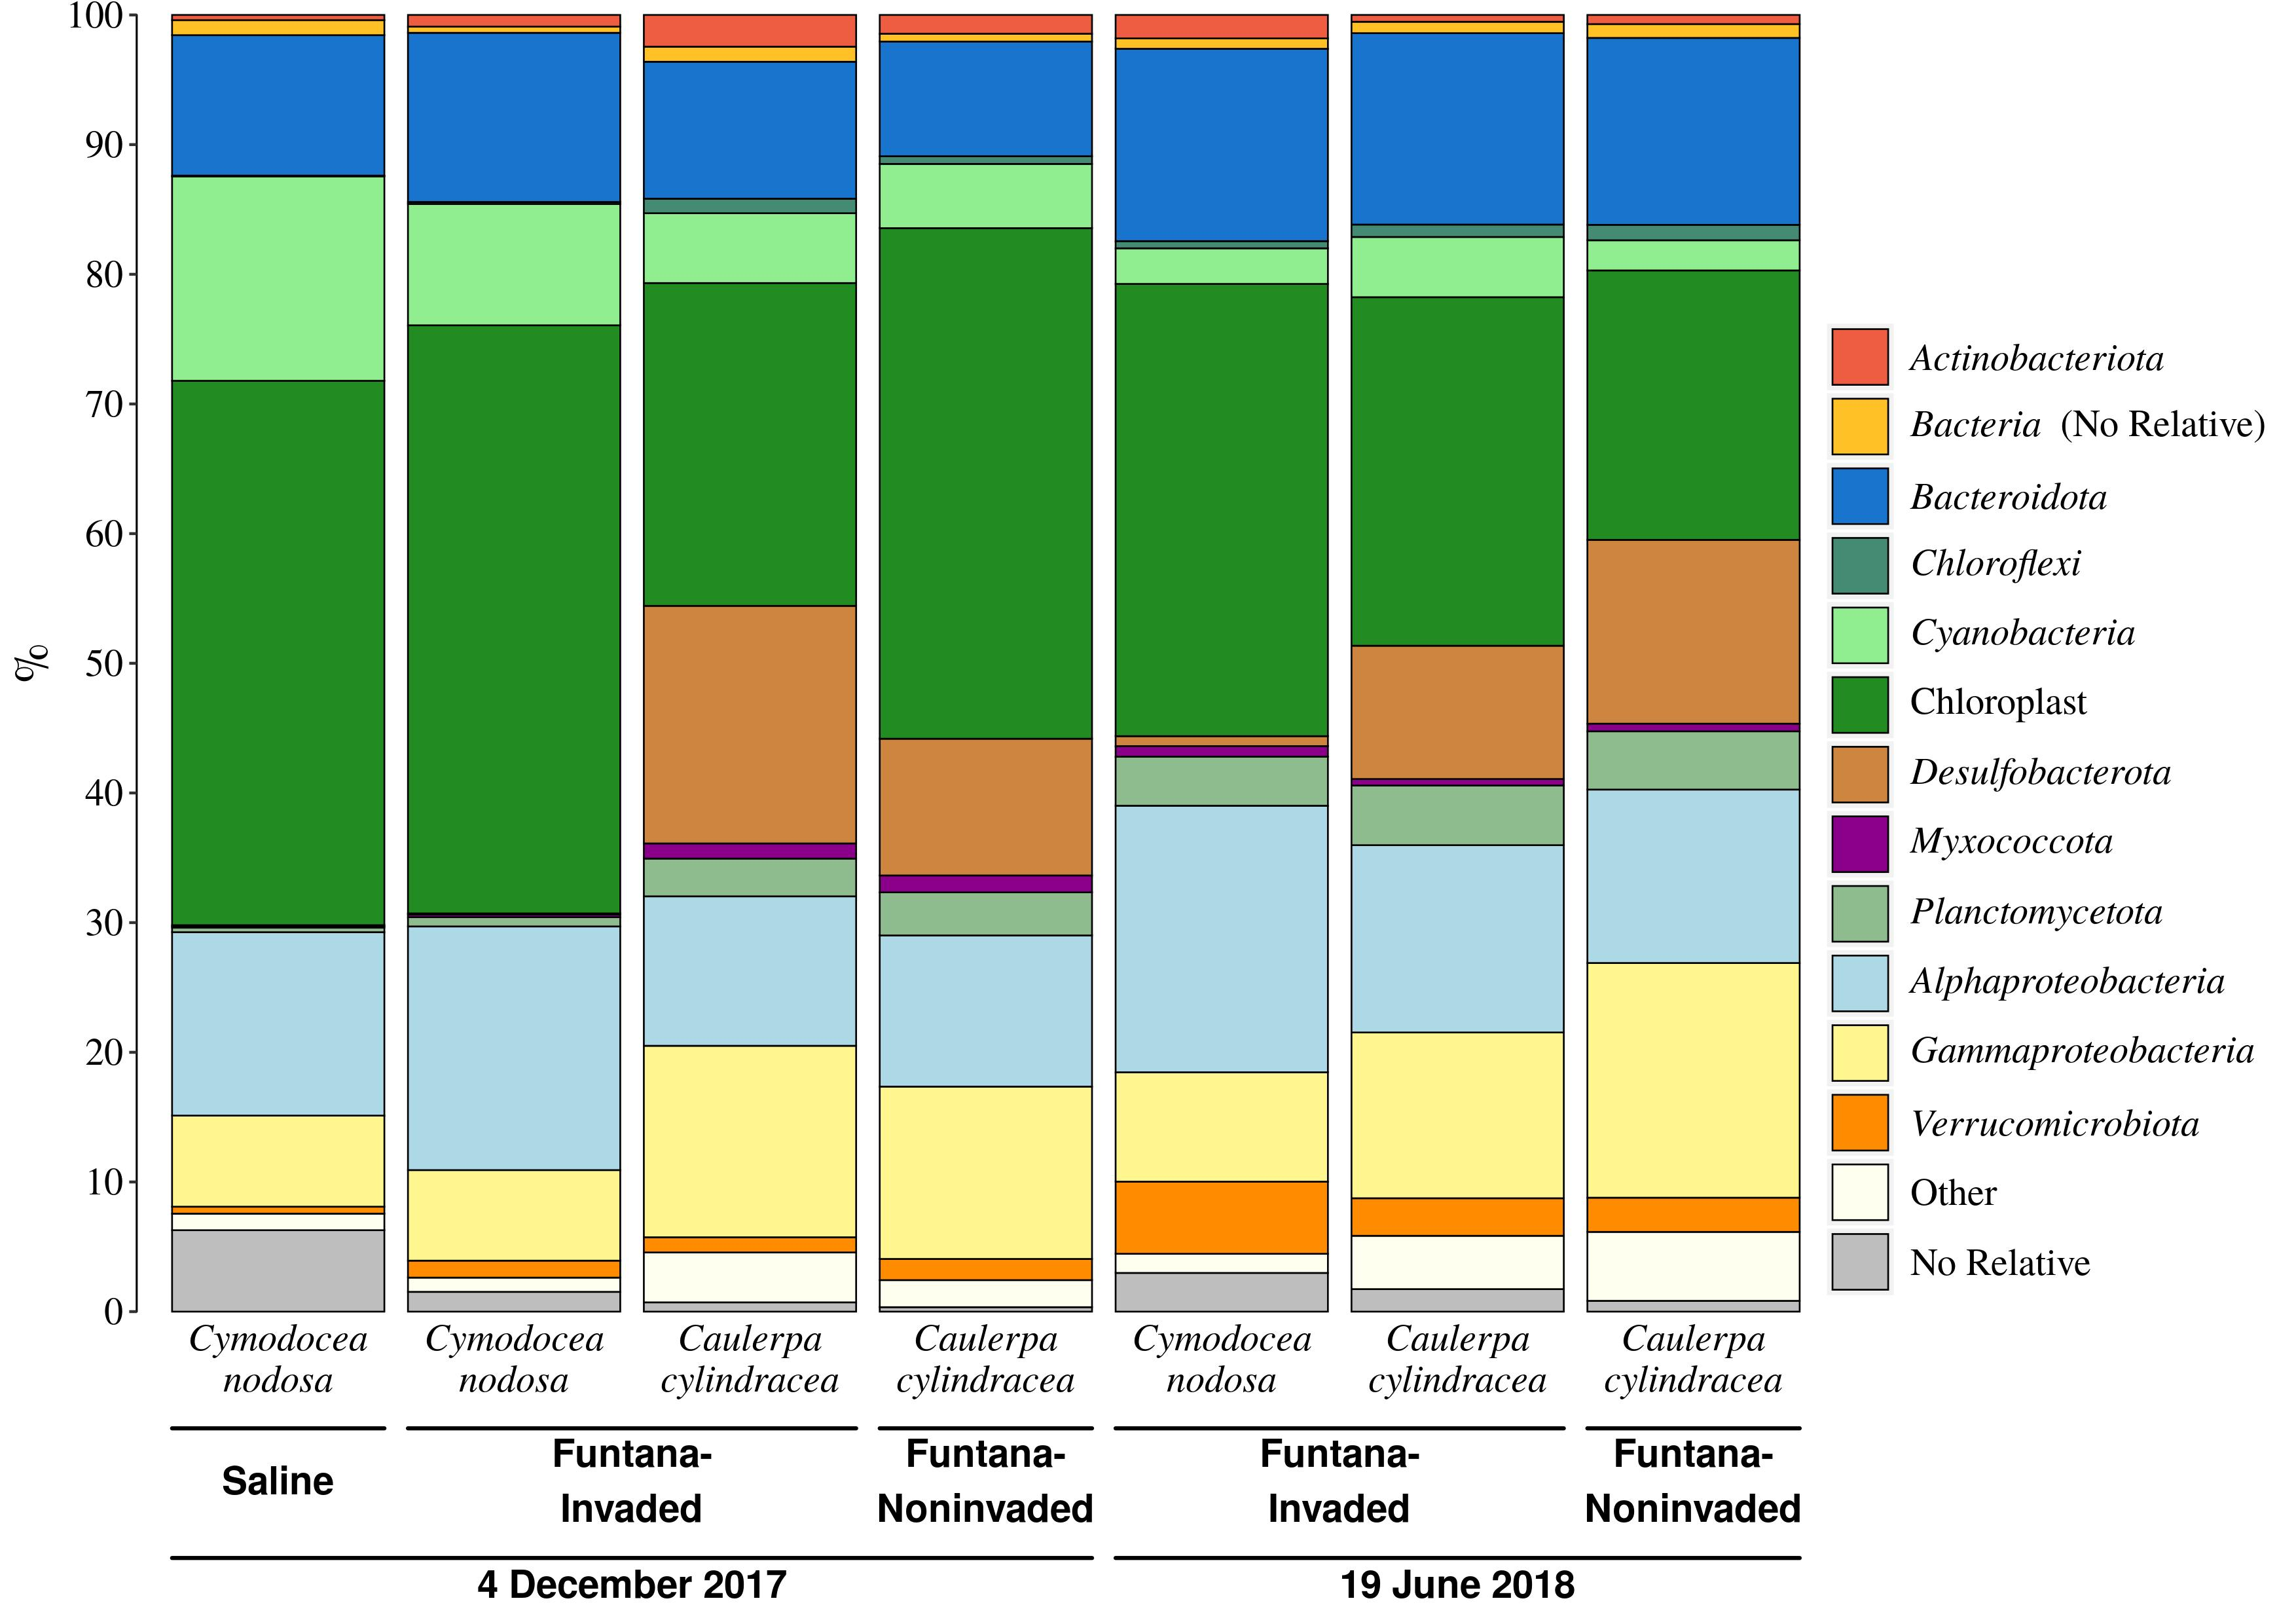
\includegraphics[width=1\linewidth]{../results/figures/community_bar_plot} 

}

\caption{Taxonomic classification and relative contribution of the most abundant (> 1 \si{\percent}) bacterial and archaeal sequences from surfaces of two marine macrophytes (\textit{C. nodosa} and \textit{C. cylindracea}) sampled in the Bay of Saline and the Bay of Funtana (Mixed and Monospecific Settlements) and in two contrasting seasons (4 December 2017 and 19 June 2018).\label{community}}\label{fig:unnamed-chunk-3}
\end{figure}

\newpage
\begin{figure}[ht]

{\centering 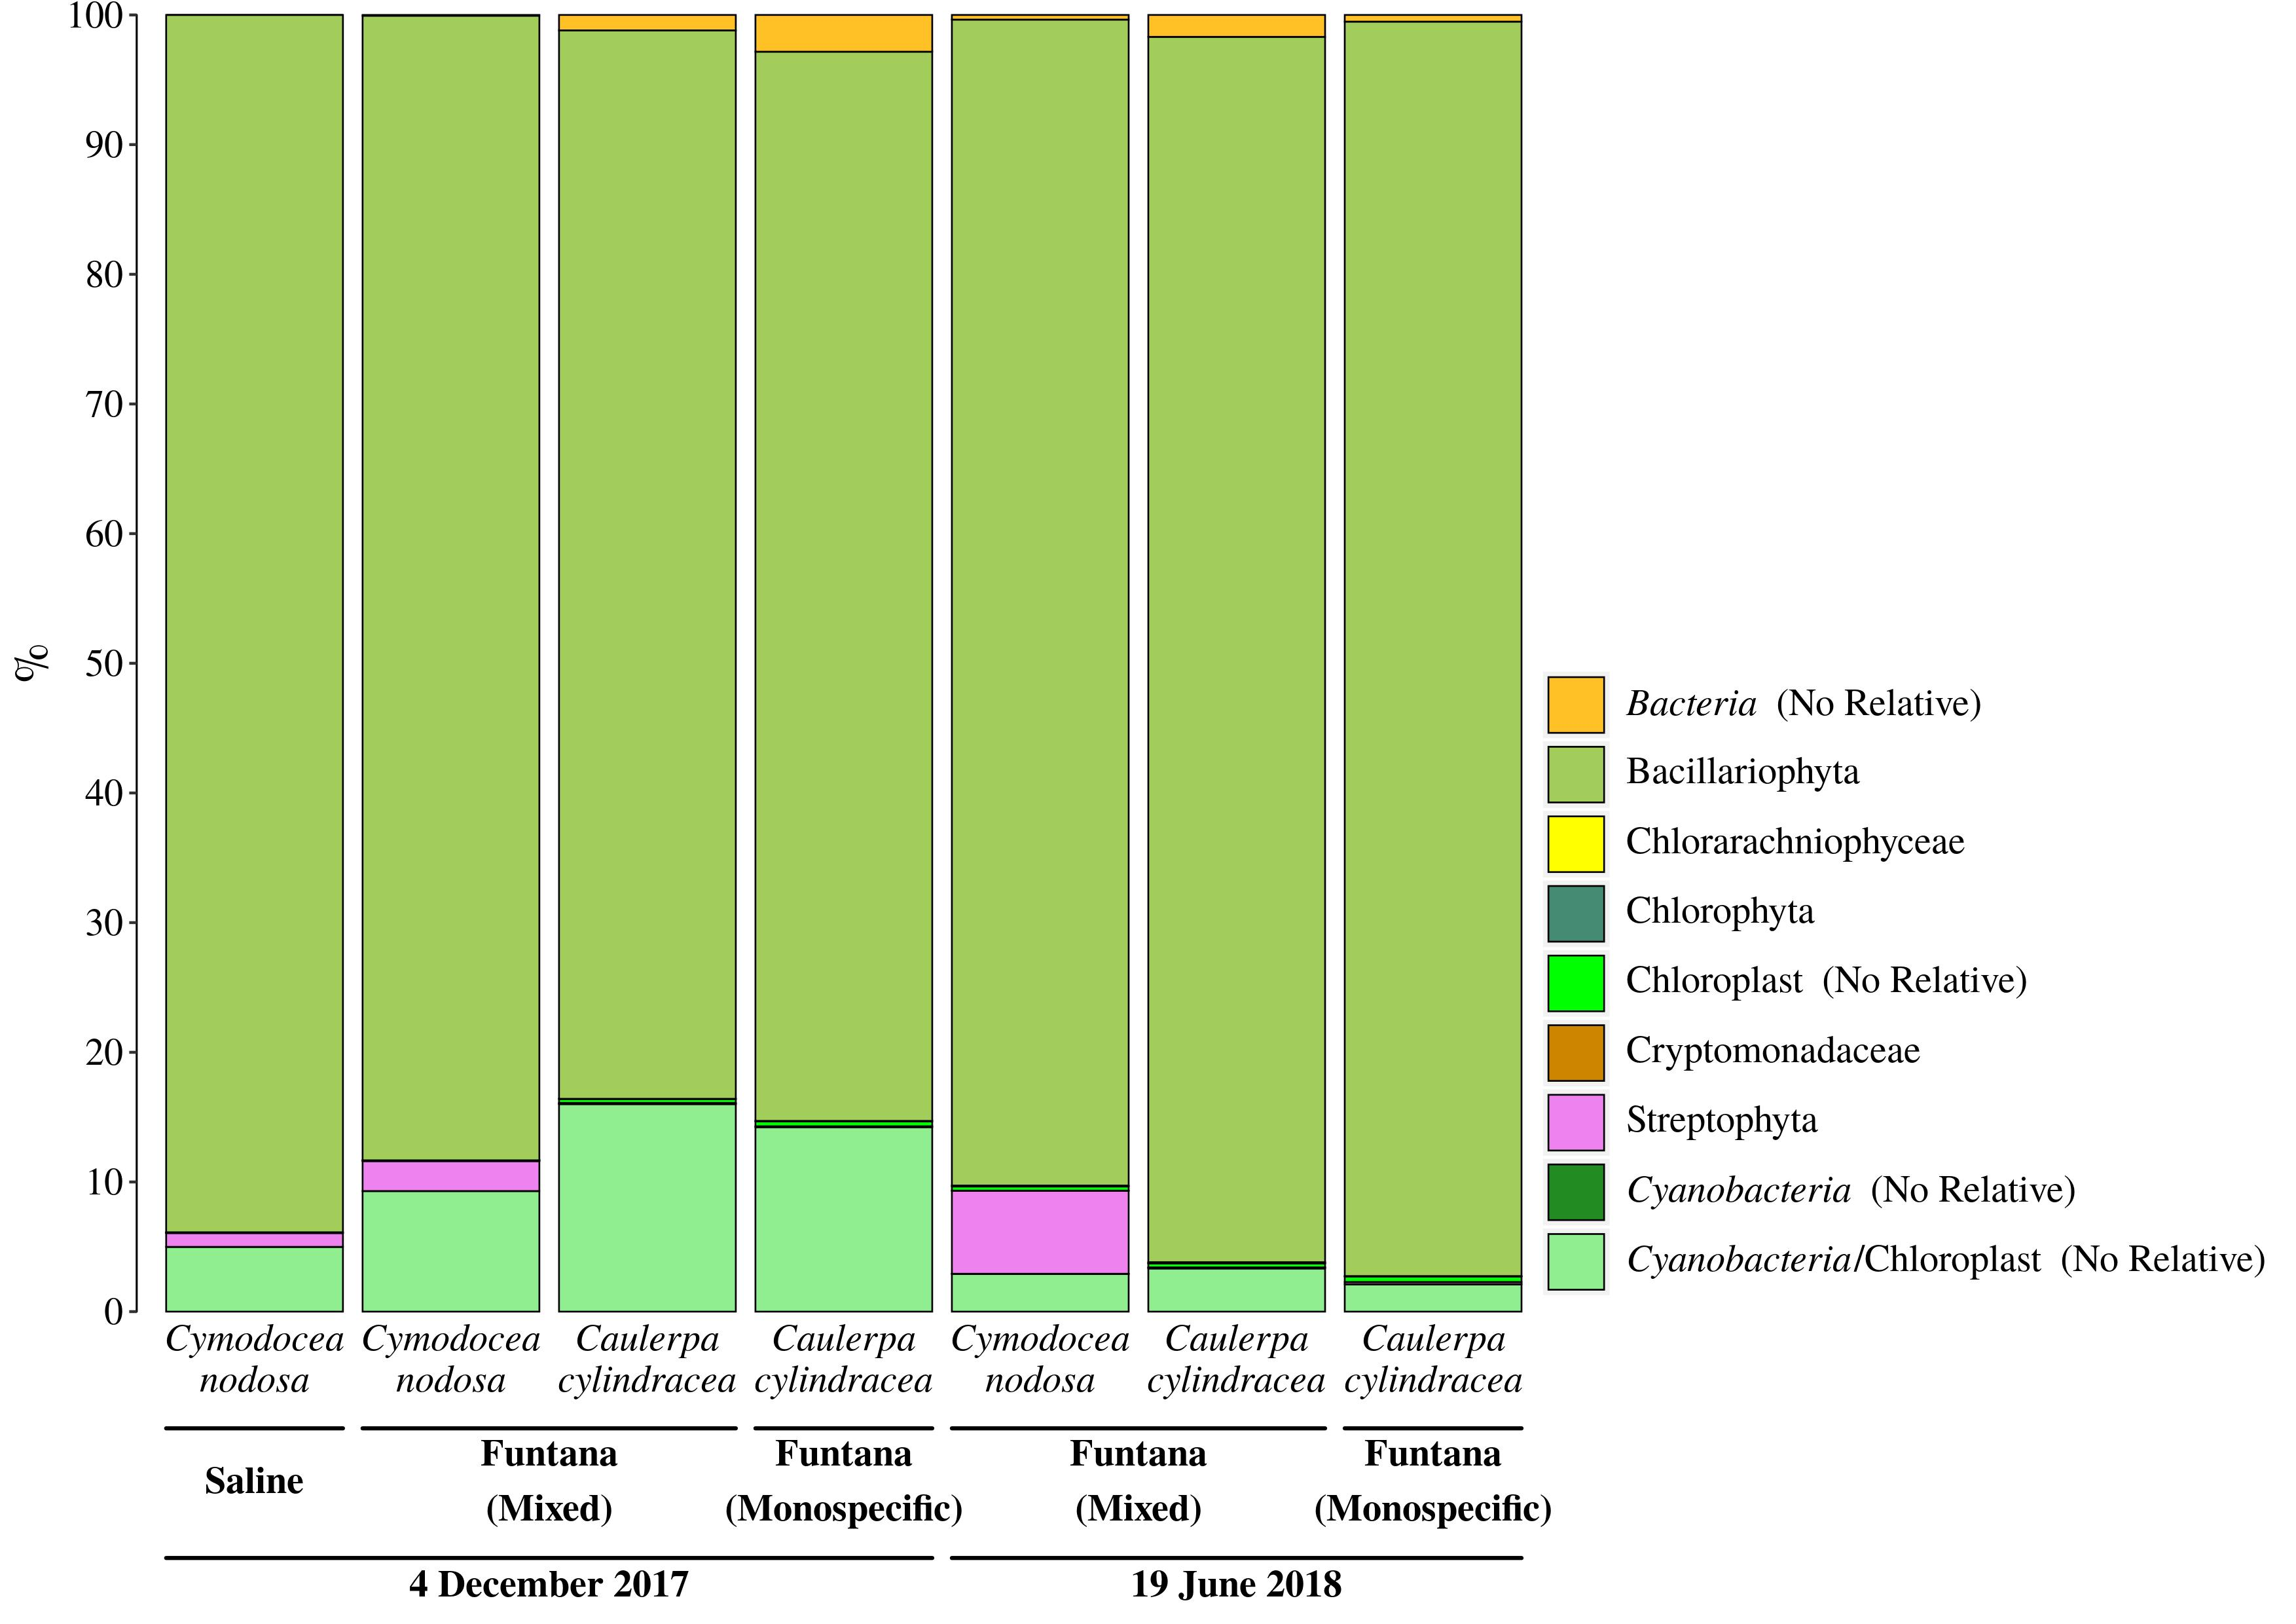
\includegraphics[width=1\linewidth]{../results/figures/chloroplast} 

}

\caption{Taxonomic classification and relative contribution of chloroplast sequences from surfaces of two marine macrophytes (\textit{C. nodosa} and \textit{C. cylindracea}) sampled in the Bay of Saline and the Bay of Funtana (Mixed and Monospecific Settlements) and in two contrasting seasons (4 December 2017 and 19 June 2018).\label{chloroplast}}\label{fig:unnamed-chunk-4}
\end{figure}

\newpage
\begin{figure}[ht]

{\centering 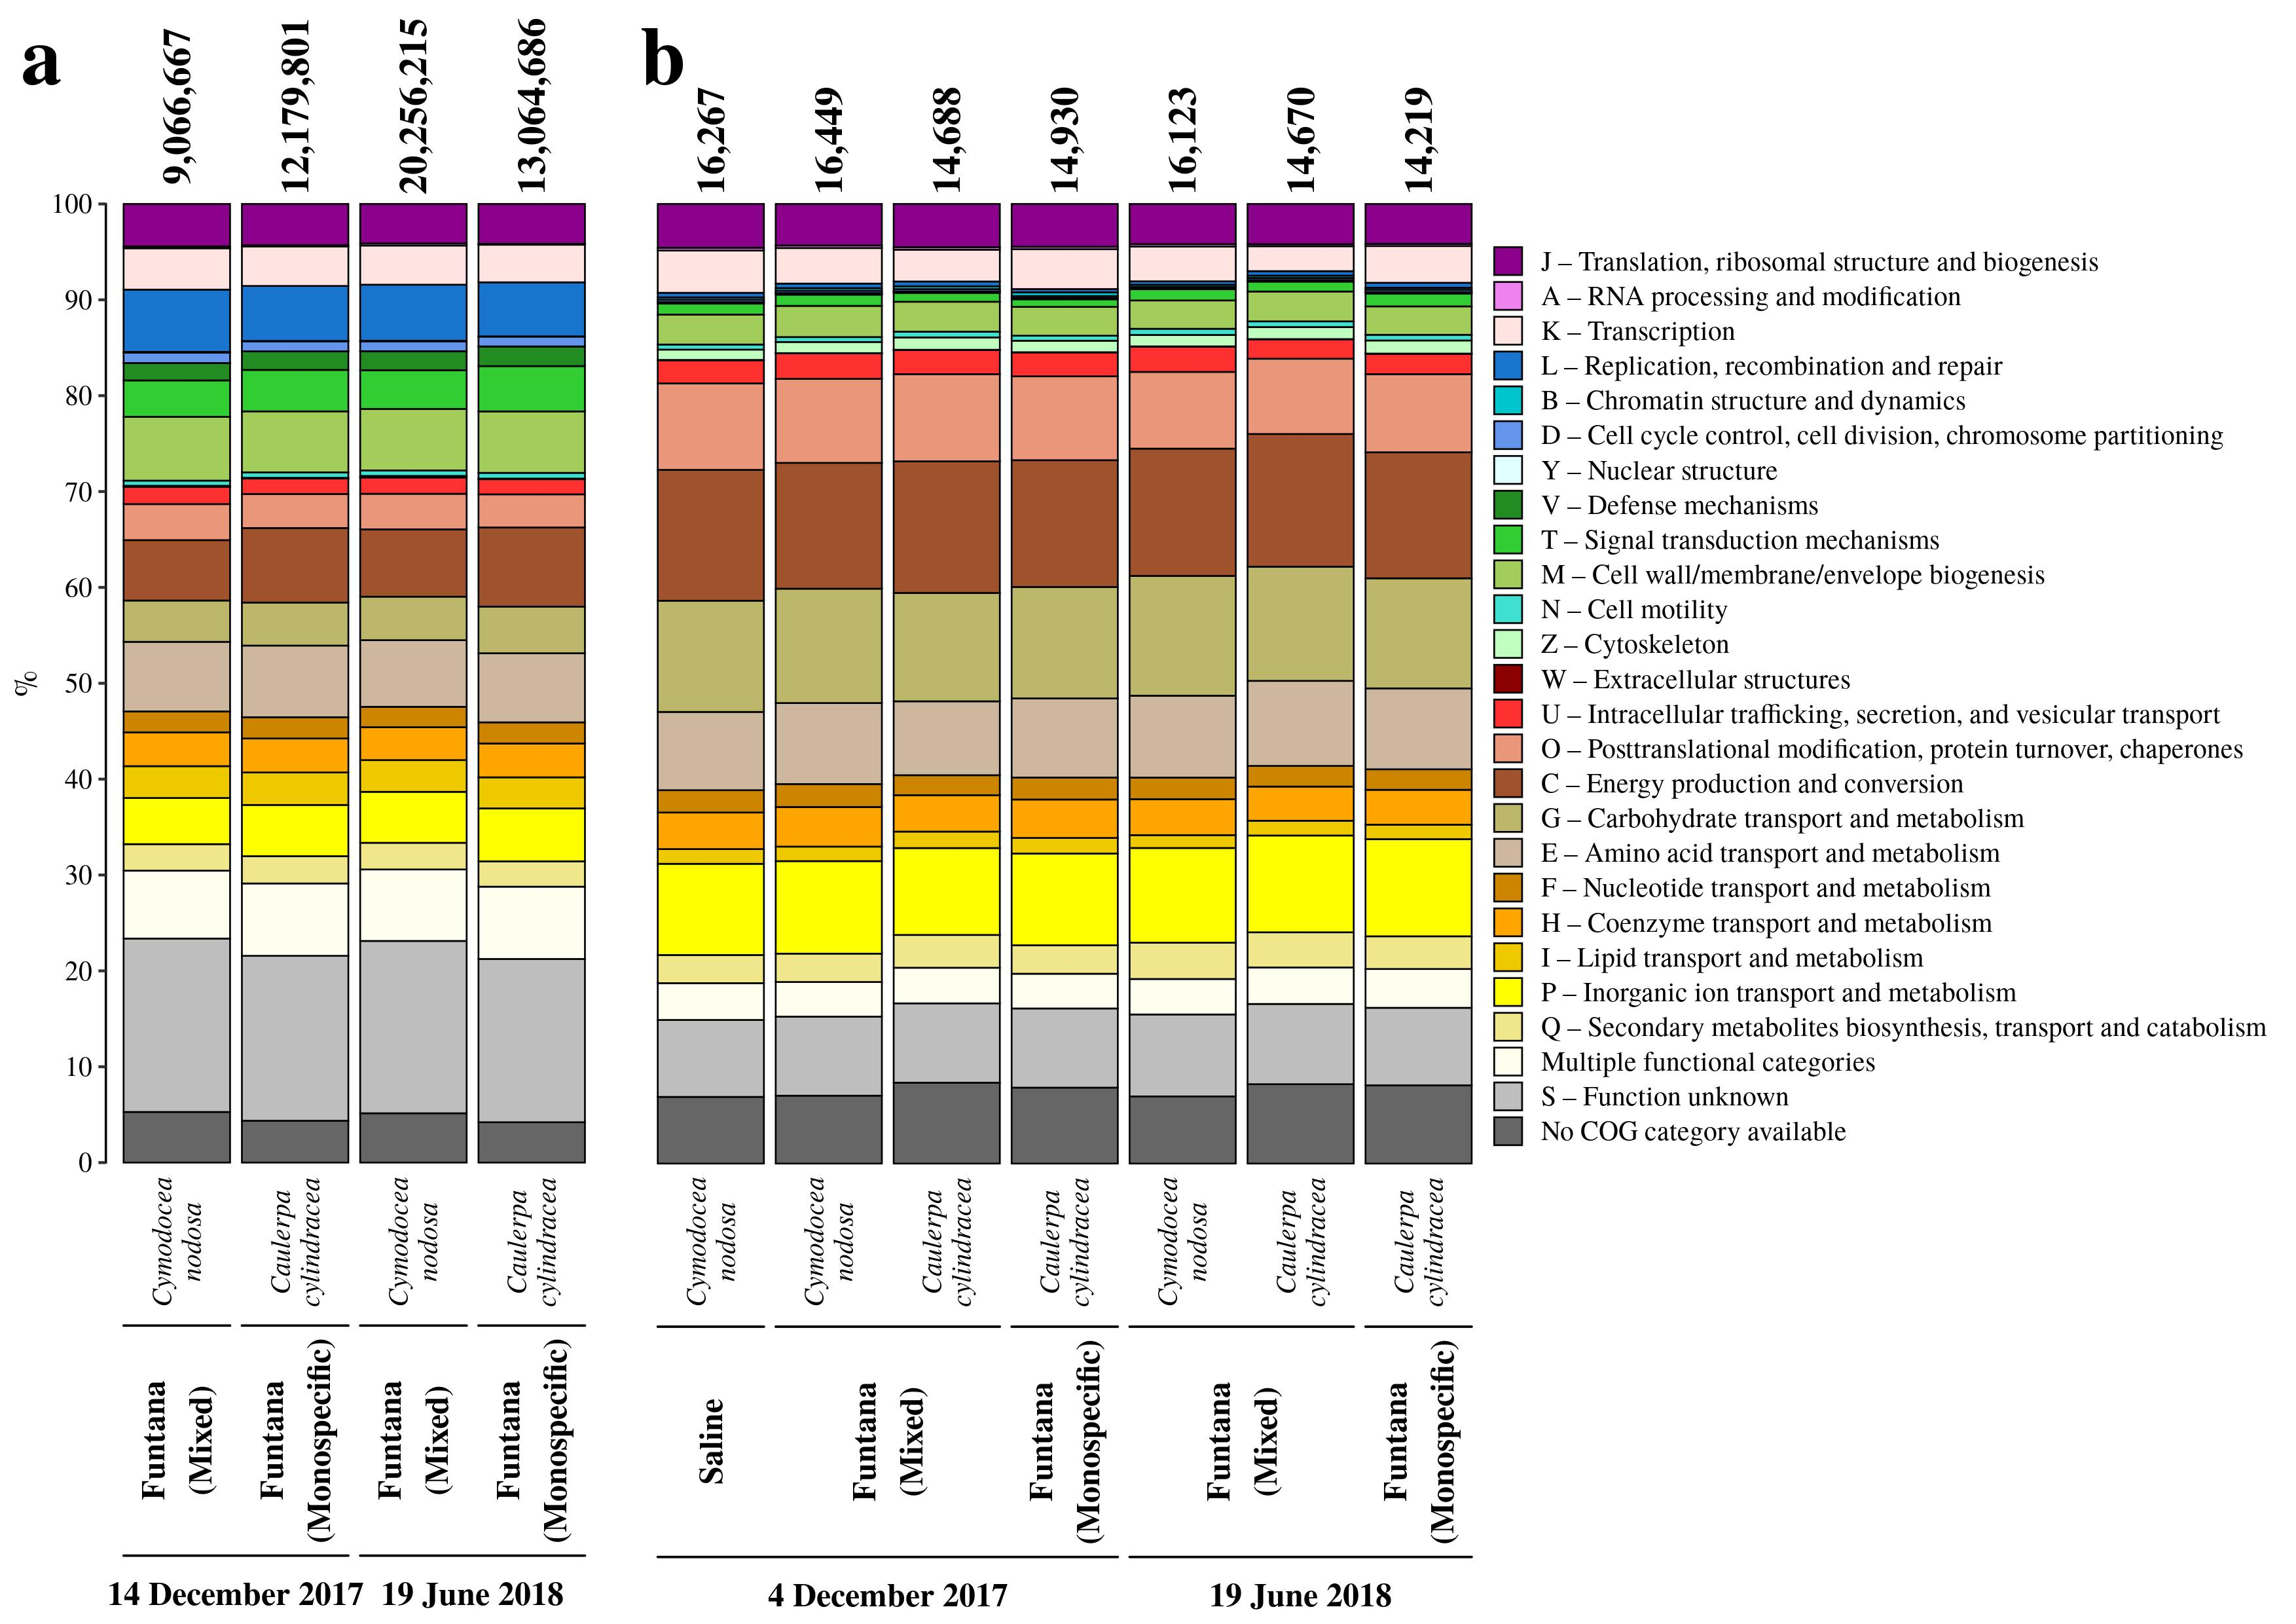
\includegraphics[width=1\linewidth]{../results/figures/cog} 

}

\caption{Relative contribution of each COG category to the total number of annotated coding sequences (A) from metagenomes and identified proteins (B) from metaproteomes associated with surfaces of two marine macrophytes (\textit{C. nodosa} and \textit{C. cylindracea}) sampled in the Bay of Saline and the Bay of Funtana (Mixed and Monospecific Settlements) and in two contrasting seasons (4/14 December 2017 and 19 June 2018). Total number of annotated coding sequences and identified proteins is given above the corresponding bar.\label{cog}}\label{fig:unnamed-chunk-5}
\end{figure}

\end{document}
